% !TeX encoding = windows-1250
\chapter{Rezultati}
%\todo[inline]{izno�enje rezultata i analiza rezultata do kojih je do�lo rje�avanjem problematike zadatka, rezultati mjerenja}
%\textit{ u poglavlju 6 �ete staviti slike i napisati rezultate zbrajanja- ne vi�e od toga.} 

\begin{figure}[!htbp]
	\begin{center}
		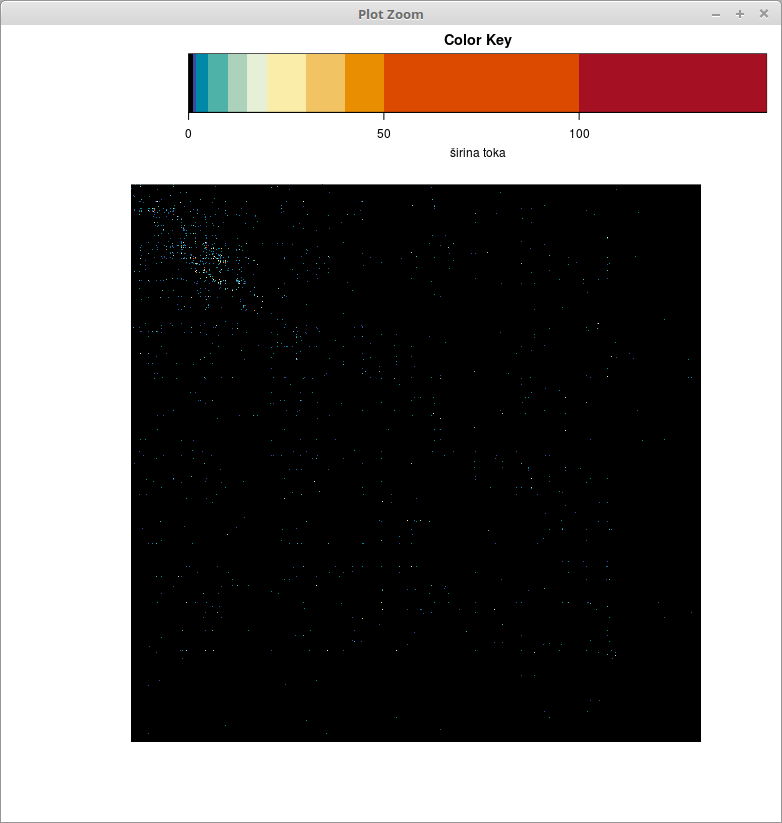
\includegraphics[width=17cm,keepaspectratio=true]{A_0_24_lmat}
		\caption{POM A}
		\label{fig:A}
	\end{center}
\end{figure}

\begin{figure}[!htbp]
	\begin{center}
		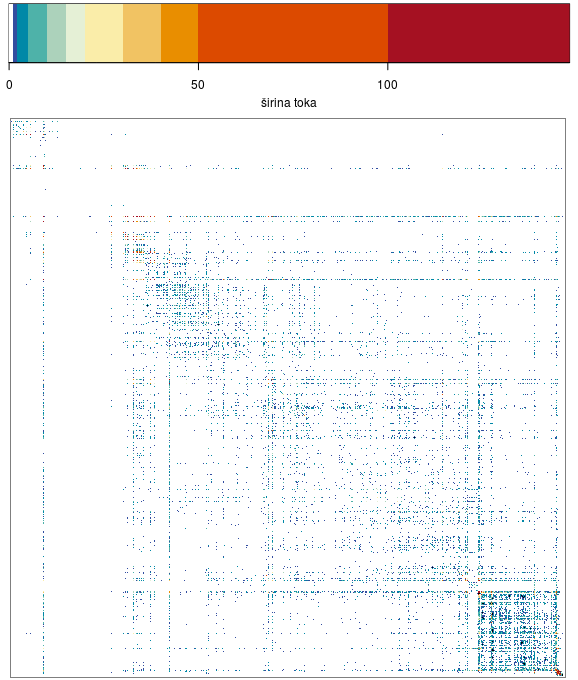
\includegraphics[width=17cm,keepaspectratio=true]{B_0_24_lmat}
		\caption{POM B}
		\label{fig:B}
	\end{center}
\end{figure}


\begin{table}[!htpb]
	\renewcommand{\arraystretch}{1.2}
	\caption{Tablica usporedbe}
	\centering
	\hskip-2.0cm
	%\tiny
	\begin{tabular}{|c|c|c|c|c|c|c|c|c|}
		\hline
		POM
		&\makecell{Prostorno\\Obuhva�anje}
		&\makecell{Gusto�a\\Informacija}
		&\makecell{Prostorna\\Zrnatost}&\makecell{Vremenska\\Zrnatost}
		%&\makecell{Tematska\\Zrnatost}
		%&\makecell{Tematska\\Rezolucija\\Svrhe}
		&\makecell{Tematska\\Rezolucija\\Na�ina kretanja}
		&\makecell{Ukupna\\�irina\\Toka}
		\\ [0.5ex]
		\hline \hline
		A&\makecell{neovisno o\\prometnoj\\infrastrukturi}
		&0.008830772
		&$1090\times1090$
		&8
		%&0
		%&0
		&0
		&30878
		\\ [0.5ex]
		\hline
		B
		&\makecell{ \\cesta\\  }
		&0.08683223
		&$1090\times1090$
		&8
		%&0
		%&0
		&1
		&427646
		\\ [0.5ex]
		\hline
		
	\end{tabular}
\end{table}
